\documentclass[12pt,a4paper]{article}
\usepackage[utf8]{inputenc}
\usepackage{graphicx} 
\usepackage{parskip} 
\usepackage{indentfirst}
\usepackage{url}
\usepackage{float}
\usepackage[spanish]{babel} % Agrega el idioma español
\usepackage{geometry} % Para ajustar los márgenes
\usepackage[T1]{fontenc}

% Configuración de los márgenes
\geometry{left=2.5cm, right=2.5cm, top=2.5cm, bottom=2.5cm}

\addto\captionsspanish{\renewcommand{\contentsname}{Contenidos}} % Cambia el nombre de la tabla de contenidos
\addto\captionsspanish{\renewcommand{\listfigurename}{Índice de figuras}} % Cambia el nombre del índice de figuras

\def\UrlBreaks{\do\/\do-}

\begin{document}

% Crear una portada personalizada
\begin{titlepage}
    \centering
    {\huge \textbf{Servidores Web de Altas Prestaciones}}\\[0.5cm]
    {\huge \textbf{Plataformas de streaming: infraestructura subyacente}}\\[0.5cm]
    {\large Tecnologías de la información}\\[0.2cm]
    Curso 2023-2024\\
    4º Ingeniería Informática\\[0.6cm]
    Nº Asignado Wiki: 14 \\[0.2cm]
    Nº de Horas: 18 horas \\[0.2cm]

    
\includegraphics[width=0.7\textwidth]{./img/logo.png}\\[1cm] % Ajusta la ruta y el tamaño según necesites
    {\Large \textbf{Integrantes del equipo:}}\\[0.5cm]
    José Luis Rico Ramos\\
    David Martínez Díaz\\
    Alejandro de la Hera Luis\\[2cm]
\end{titlepage}

% Índice
\tableofcontents
\newpage

% Índice de figuras
\listoffigures
\newpage

% Introducción
\section{Introducción}

En las últimas décadas, se ha producido una revolución en cómo vemos y consumimos el contenido multimedia a través de las plataformas de streaming, los cuales permiten que podamos ver películas y escuchar música a través de internet, donde prácticamente se ha convertido en parte de nuestra día a día.

Por tanto, toda esta revuelta ha conseguido desplazar a los medios de comunicación tradicionales como la televisión y la radio, haciendo que cada vez se escuchen menos, dando paso a una nueva era en el entretenimiento y en la información. Esta nueva era, no solo cambia la manera en la que vemos el nuevo contenido, sino que también ha redefinido las industrias creativas e innovadoras, generando nuevas oportunidades y desafíos.

Con este trabajo se pretende tanto explorar cómo explicar los distintos funcionamientos a nivel interno de los servicios de streaming, destapando sus tecnologías y estrategias que les permiten a estas plataformas ofrecer amplios catálogos de contenido a la carta y siendo rentables.

También se quiere comparar las distintas plataformas a nivel de estructura operativa y de negocio, sobre todo de los líderes de mercado, para identificar las claves de su éxito en un entorno altamente competitivo. Con esta búsqueda de información, queremos mostrar sobre dichas estrategias tomadas por las plataformas de streaming en un ámbito global y ver su impacto en el consumo de medios digitales.

Por lo que la estructura a seguir en este trabajo se divide en varias partes, primero proporcionaremos una visión general general de la evolución de las plataformas, luego examinaremos en detalles la tecnología utilizada detrás del streaming. Luego realizaremos un análisis comparativo entre las principales plataformas, sobre todo a nivel de estructura.

Por último, comentaremos las conclusiones obtenidas sobre dichas comparaciones y reflexionaremos sobre los componentes clave para poder estar entre las plataformas más grandes.
\newpage

\section{Antecedentes o preliminares}
En primer lugar, empezaremos definiendo qué son en sí las plataformas de streaming, estas son servicios digitales que permiten a los usuarios acceder a una gran cantidad de contenido multimedia, desde películas, series y música hasta eventos en vivo sin la necesidad de descargar nada, simplemente a través de internet.

El funcionamiento de estos servicios se basa en el modelo de transmisión continua de datos, siempre intentando adaptarse a las velocidades de conexión que disponga el usuario, para poder ofrecer la mejor calidad posible en resolución y reproducción en tiempo real. Entre las características que debe tener estos tipos de servicios podemos mencionar los siguientes:

\begin{itemize}
    \item \textbf{Acceso inmediato}: Los usuarios deben poder ver o escuchar el contenido que hayan elegido al momento, intentando reducir los tiempos de espera lo máximo posible.
    \item \textbf{Gran catálogo}: Las plataformas deben ofrecer una gran cantidad de opciones y bibliotecas de contenido, con diferentes géneros, categorías y formatos.
    \item \textbf{Personalización}: Los usuarios deben poder tener un perfil basado en las preferencias y en el contenido consumido, para ello se utilizan algoritmos para recomendar según los perfiles personalizados de cada usuario.
    \item \textbf{Flexibilidad}: Es importante la accesibilidad a la aplicación, independientemente del dispositivo utilizado, ya sea un smartphone, una tablet o un portátil, siempre y cuando estén conectados a internet.
    \item \textbf{Modelos de pago}: Lo más frecuente es utilizar modelos de suscripción (mensuales, anuales, etc.), pero también existen otras alternativas como variantes con publicidad o de compras únicas.
\end{itemize}

El origen de los streaming empezó alrededor de 1990, pero no fue hasta mediados de los 2000 que las plataformas de streaming empezaron a ganar popularidad y a tomar forma, debido principalmente a la mejora en las velocidades de conexión a internet y sobre todo a la aparición de tecnologías de compresión de datos. En un inicio, estos servicios eran muy limitados, ya que los contenidos que ofrecían eran muy escasos y siempre había problemas técnicos.

Sin embargo, conforme iba pasando el tiempo estos servicios se han ido convirtiendo poco a poco en gigantes del entretenimiento y la información, donde ahora se ofrecen desde series y películas que han sido producidas exclusivamente para sus propias plataformas hasta eventos deportivos de escala internacional en vivo. Dicha evolución ha estado definida sobre todo por la innovación tecnológica, la expansión global y la adaptación a las necesidades de los usuarios.

\newpage

Principalmente existen dos tipos de servicio de streaming, que han surgido para satisfacer diferentes necesidades de los usuarios a la hora de consumir contenido:

\begin{itemize}
    \item \textbf{Streaming en directo (Live streaming)}: Esta función permite transmitir eventos en tiempo real y facilitar que los usuarios sean parte de una experiencia simultánea con otras audiencias en cualquier parte del mundo. Las transmisiones en directo son muy populares en eventos deportivos, conciertos y transmisiones en vivo de creadores de contenido compartidas en redes sociales.
    \item \textbf{Streaming “on-demand”}: Gracias a esta función, los usuarios pueden disfrutar de una colección de contenido pregrabado en cualquier momento. Esta es la modalidad más popular para plataformas de series, películas y documentales, ya que es altamente flexible y adaptable a la personalización de contenido.
\end{itemize}
\newpage

\section{Objetivos}

La finalidad de este trabajo realizado es poder comprender y mostrar a fondo cómo es la infraestructura de las plataformas de streaming más importantes del sector. Con este documento se busca explicar tanto los mecanismos como las tecnologías utilizadas para poder afrontar las dificultades en el consumo de contenido digital.

Por ello, intentaremos centrarnos sobre todo en las estructuras de datos, en los sistemas de carga de red y las soluciones implementadas para el almacenamiento y la recuperación de datos para poder intentar entender cómo se sostiene este modelo de negocio.

Además, se hará un análisis sobre cómo las plataformas manejan los volúmenes de datos y el tráfico en tiempo real. Por otro lado, también se podrá observar las técnicas de balanceo de carga, los CDN y otras estrategias que facilitan sobre todo la transmisión eficiente de contenido multimedia a una gran cantidad de usuarios a la vez.

Entre otros objetivos a cumplir, podemos mencionar la comparación entre las distintas implementaciones de las plataformas líderes como son Netflix, Amazon Prime Video y Youtube, con el propósito de poder identificar las prácticas más efectivas e innovadoras, también servirá para poder ver tanto las diferencias en las arquitecturas como sus similitudes.

Por último, se hará una pequeña evaluación de cómo es el impacto de estas tecnologías en la experiencia del usuario final, para poder ver aspectos importantes como la infraestructura tecnológica con aspectos como la calidad de video, la rapidez de acceso al contenido, la personalización de la experiencia... etc.

\newpage


\section{Infraestructura subyacente de las plataformas de streaming}
Si comenzamos a hablar sobre la infraestructura de las plataformas de streaming, lo primero que se nos viene a la cabeza es la complejidad en su diseño para poder hacer frente a la transmisión de grandes cantidades de datos de una manera eficiente y sobre todo en tiempo real a usuarios de todo el mundo.

Si queremos ver más de cerca cómo funcionan dichas infraestructuras, podemos definir los componentes más básicos que cualquier servicio de este tipo debe tener, así como el funcionamiento general de estos y los posibles retos a enfrentar:

\begin{itemize}
    \item \textbf{Servidores}: Esta es la parte esencial de cualquier plataforma de streaming, ya que deben ser unos servidores potentes para que sean capaces de almacenar el contenido multimedia y de procesarlos para hacer su transmisión, además suelen estar repartidos estratégicamente por todo el mundo para así hacer frente a los problemas de latencia.
    \item \textbf{Redes de Distribución de Contenidos (CDN)}: La red de distribución de contenidos (CDN) es una red global de servidores que optimiza la entrega de contenidos almacenando múltiples copias de los mismos en servidores geográficamente dispersos, lo que garantiza que el contenido se obtiene siempre del servidor más cercano. De ahí el aumento de la carga y la disminución de la latencia.
    \item \textbf{Sistemas de almacenamiento}: Con el gran volumen de contenidos que circulan por estas plataformas, los sistemas de almacenamiento desempeñan un papel fundamental a la hora de gestionar y garantizar el fácil acceso a los contenidos. Incluye las soluciones de almacenamiento en la nube y el almacenamiento físico.
    \item \textbf{Codificadores de vídeo}: Son herramientas que transcodifican la grabación original a un formato de archivo optimizado para streaming y adaptan la calidad del vídeo a la capacidad de ancho de banda del usuario.
    \item \textbf{Gestión de Derechos Digitales (DRM)}: Sistemas de protección de contenidos multimedia que se supone que ayudan a proteger el material protegido por derechos de autor contra todo tipo de usos indebidos.
\end{itemize}

El proceso de streaming comienza con la compresión y codificación del contenido multimedia en un formato adecuado para su transmisión por Internet, y este es conducido y almacenado en los servidores. Una vez hecho este paso, está listo para ser distribuido a través de las CDN.

El proceso que se sigue para ver un video es el siguiente, cuando el usuario lo solicita el sistema se encarga de determinar cuál es el servidor CDN más cercano y cuál es la mejor calidad y resolución del video en función del ancho de banda que se disponga, teniendo en cuenta los protocolos de transmisión más comunes como HLS (HTTP Live Streaming) y MPEG-DASH. Lo que hacen dichos protocolos es dividir principalmente el contenido en paquetes más pequeños, consiguiendo una transmisión fluida y que sea flexible, así se puede ajustar la calidad del video a las condiciones que haya en el momento del traspaso de la información.

Por último, comentar los posibles retos técnicos que nos podemos encontrar a la hora de desplegar las plataformas de streaming:

\begin{itemize}
    \item \textbf{Latencia}: Para reducir el tiempo de entrega de los contenidos, estas plataformas utilizan CDN y optimizan los algoritmos de enrutamiento. También adoptan la tecnología de edge computing (computación de borde) de procesamiento de datos más cercana al usuario final.
    \item \textbf{Escalabilidad}: Las demandas pico de los usuarios pueden sobrecargar los sistemas. Las soluciones en la nube y la arquitectura distribuida de las CDN permiten escalar recursos rápidamente, según sea necesario.
    \item \textbf{Seguridad}: Ante todo, a las plataformas lo que más les preocupa es la seguridad de los contenidos y datos de sus usuarios, para lidiar con esto utilizan herramientas como DRM y el cifrado de datos, consiguiendo así integrar protocolos de seguridad de una manera sólida.
    \item \textbf{Gestión del ancho de banda}: Hay que tener en cuenta el ancho de banda para la gestión de la calidad del contenido en streaming, ya que hay que buscar un equilibrio entre la resolución de las imágenes que se traspasan según el ancho de banda que tengamos disponible, así garantizamos un streaming fluido aunque haya conexiones que no sean estables y uniformes.
\end{itemize}

\newpage

\section{Desarrollo de las infraestructuras de distintas plataformas}
En este análisis, seleccionaremos tres de las plataformas de streaming más populares y reconocidas a nivel mundial: Netflix, Amazon Prime Video y Youtube. 

Donde cada una de estas plataformas ha conseguido liderar el mercado del entretenimiento digital con su respectivo enfoque único y con estrategias tecnológicas que le dan color a su servicio.

Iremos viendo la infraestructura uno por uno, comentando sus características y los componentes y estrategias que optan para gestionar todo el contenido multimedia y la manipulación de la información.

    \subsection{Netflix}

    \subsubsection{Diseño de alto nivel}

    Para ver desde una perspectiva general y amplia cómo es la infraestructura de Netflix, considerada como una de las más grandes plataformas de streaming, primero debemos analizar cómo está diseñada para cumplir con una serie de requisitos tanto funcionales como no funcionales, que garanticen una experiencia de usuario completa y satisfactoria. 

    Entre los requisitos funcionales, como en cualquier plataforma web, destaca la gestión de usuarios, la reproducción avanzada que otorgue a los usuarios control total sobre la visualización, incluyendo funciones como pausar, rebobinar y descargar para ver offline. Por último, mencionar las recomendaciones personalizadas, otra de las claves de su éxito, ya que se ajustan a las preferencias individuales de cada usuario, mejorando así la retención y satisfacción del cliente.

    En cuanto a los no funcionales, la arquitectura de Netflix ha sido diseñada para mantener un rendimiento óptimo, consiguiendo obtener una capacidad de respuesta decente aun habiendo grandes cargas en el tráfico. La alta disponibilidad y la seguridad también son fundamentales, teniendo especial cuidado en la autenticación de los usuarios y en su respectiva autorización, ya que para Netflix es muy importante proteger a los usuarios y a sus datos, compaginando todo con una interfaz intuitiva y fácil de navegar. \cite{adm2023}

    A nivel global, podemos definir la infraestructura de Netflix según tres componentes, siendo el primero de ellos el Cliente, que representa la interfaz con la que los usuarios interactúan. Seguido tenemos el “Open Connect”, que es la red de distribución de contenido personalizada y por último tenemos el Servidor, que abarca todo el back-end y que se gestiona principalmente por Amazon Web Services (AWS). \cite{boettger2018}

    Por tanto, vemos que el núcleo de la infraestructura está compuesta principalmente por dos nubes, AWS (Amazon Web Services) y Open Connect, con lo que consigue hacer una entrega eficiente del contenido que ofrecen. En AWS es donde está alojado el servidor backend, donde se encuentra la lógica de negocio, la gestión de usuarios, el procesamiento de datos y el resto de funciones que no están relacionadas directamente con la transmisión de video. 
    
    Por otro lado, tenemos a Open Connect, que es el que se encarga de optimizar la entrega de los videos a los usuarios, distribuyendo dicho contenido por una red de servidores ubicados estratégicamente alrededor del mundo. Con esto se consigue hacer frente al primer reto de la latencia, al poder servir los datos desde una ubicación más cercana al usuario, consiguiendo así una experiencia de alta calidad sin interrupciones.

    \begin{figure}[H]
        \centering
        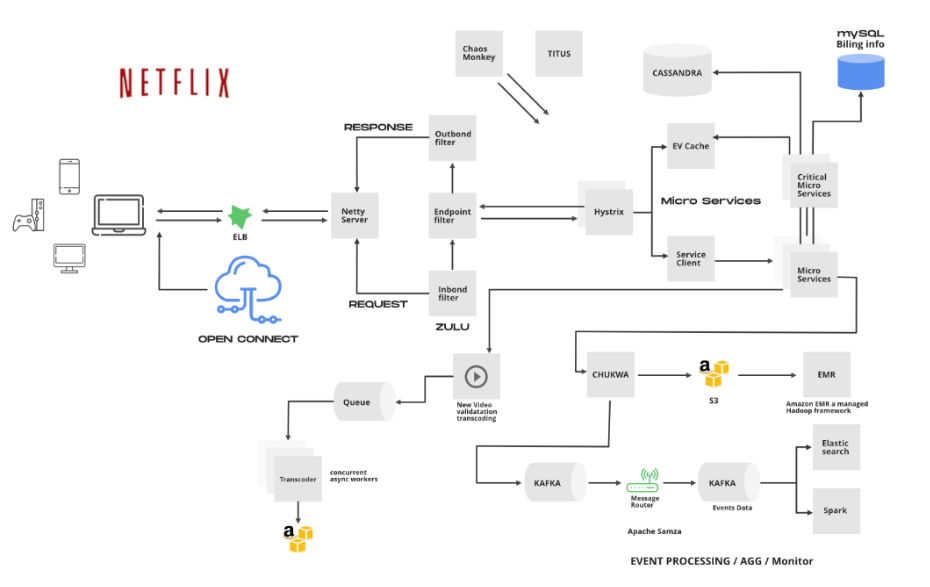
\includegraphics[width=0.8\textwidth]{./img/infraestructura_netflix.png}
        \caption{Infraestructura general de Netflix}
        \label{fig:netflix_infra}
    \end{figure}


    \subsubsection{Arquitectura de microservicios de Netflix}

    Si hablamos de la infraestructura de Netflix, hay que mencionar la arquitectura de microservicios que tiene, ya que descompone la aplicación en una serie de servicios independientes, donde cada servicio ejecuta su propio proceso y se comunican entre sí a través de interfaces ligeras (HTTP API).

    Cuando un usuario realiza una solicitud, entra en un ecosistema de microservicios, donde se redirige dicha solicitud entre los diferentes microservicios que tengan una tarea asignada a dicha petición, como la autenticación o la reproducción de un video. Además, dichos servicios pueden comunicarse entre sí, originando así un flujo de datos pero que siempre termina en una respuesta “íntegra”. \cite{gfg2024b}

    \begin{figure}[H]
        \centering
        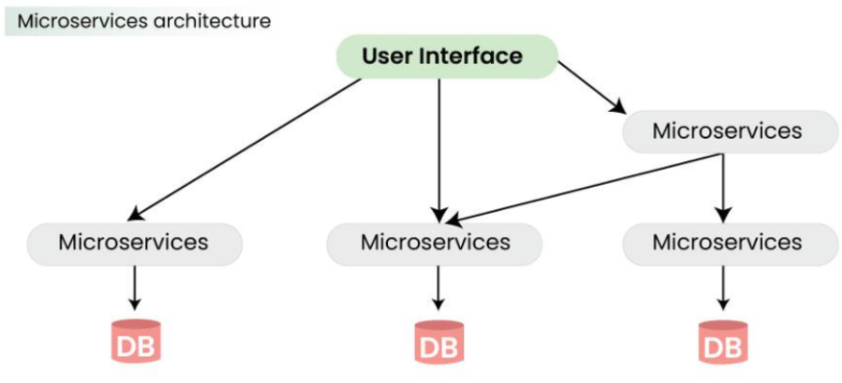
\includegraphics[width=0.8\textwidth]{./img/arquitectura_microservicios_netflix.png}
        \caption{Arquitectura de Microservicios de Netflix}
        \label{fig:netflix_microservices}
    \end{figure}

    Aun así, para asegurar que la arquitectura sea confiable, Netflix posee una serie de herramientas específicas, por ejemplo, el uso de Hystrix que se trata de un controlador de tolerancia a fallos y que además protege al sistema en contra de las interrupciones, consiguiendo así que aunque ocurra algún fallo no se comprometa la estabilidad del sistema.

    Una característica a mencionar es que Netflix promueve la separación de microservicios críticos, es decir, aquellos que son esenciales para las necesidades básicas del usuario, como la búsqueda y la reproducción de contenido. Esto se hace con la finalidad de que dichos servicios tengan una alta disponibilidad y sean bastante resistentes a fallos, intentando depender lo más mínimo de otros servicios, para que cuando haya fallos sistémicos, aunque sea que las funcionalidades más importantes estén operativas.

    Netflix también adopta un enfoque de "servidores como ganado, no como mascotas", ya que realmente son recursos intercambiables, por lo que si un servidor falla o empieza a bajar su rendimiento, puede ser cambiado sin afectar a las operaciones del servicio, consiguiendo así facilitar la escalabilidad horizontal.

    \subsubsection{Diseño de bajo nivel del sistema}

    Si nos adentramos a un nivel más bajo en la infraestructura, podemos ver que Netflix empieza sus procesos de incorporar contenido recibiendo videos de alta calidad y dado que la plataforma es accesible desde prácticamente cualquier dispositivo (2.200 dispositivos distintos), cada uno con sus propios requisitos específicos de resolución y formato, es importante realizar un preprocesamiento coherente y eficaz.

    Dicho preprocesamiento incluye la transcodificación de los videos originales a diferentes formatos y resoluciones, para garantizar la compatibilidad con la mayoría de los dispositivos pero también para optimizar la experiencia de visualización ajustando la calidad del video según la velocidad de conexión que posea el usuario.

    \begin{figure}[H]
        \centering
        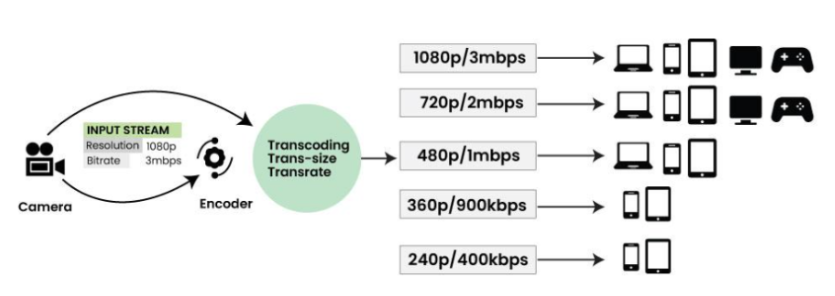
\includegraphics[width=0.8\textwidth]{./img/transcodificacion_netflix.png}
        \caption{Transcodificación de los videos originales}
        \label{fig:netflix_transcoding}
    \end{figure}

    Para lograr esto, Netflix crea alrededor de 1100 réplicas de cada una de las películas que incorpora a su sistema, cada una de ellas con una resolución distinta. Este proceso se lleva a cabo en el servidor alojado en AWS, donde el video original se divide en fragmentos más pequeños que luego son convertidos a diferentes formatos.

    Dichos archivos procesados son repartidos a través de la red global de servidores de Open Connect, lo que permite que los usuarios siempre tengan acceso al contenido desde la ubicación más cercana.

    Para hacer frente a la alta carga de tráfico, Netflix utiliza diferentes tecnologías, como el Equilibrador de Carga Elástico (ELB) de AWS, que se encarga de distribuir el tráfico entre las zonas y los servidores disponibles utilizando un esquema de equilibrio de cargas basado en Round-Robin y DNS.

    \begin{figure}[H]
        \centering
        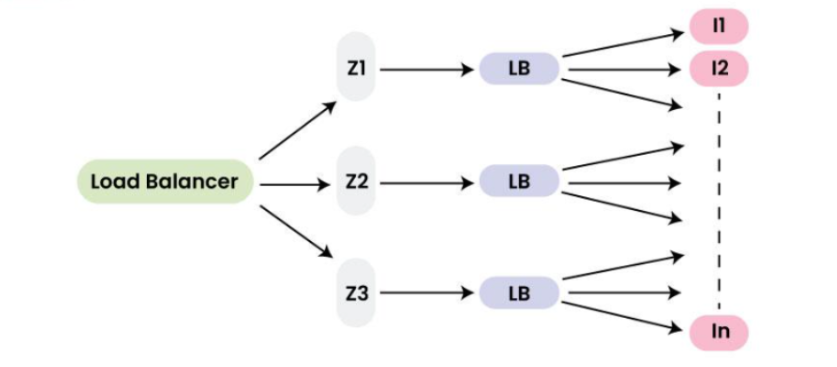
\includegraphics[width=0.8\textwidth]{./img/equilibrador_carga_elastico_netflix.png}
        \caption{Equilibrador de Carga Elástico (ELB)}
        \label{fig:netflix_elb}
    \end{figure}

    Por otro lado, también utilizan ZUUL como puerta de enlace proporcionando enrutamiento dinámico, monitoreo y seguridad. Al filtrar y dirigir las solicitudes de los usuarios a los servicios correspondientes, facilita la administración del tráfico y mejora la resiliencia de la plataforma frente a fallos o sobrecargas en ciertos componentes del sistema. \cite{hoff2018}

    Con el fin de mejorar el rendimiento y la disponibilidad de su aplicación, Netflix ha desarrollado un almacenamiento en caché conocido como "caché EV" basado en Memcached, que permite almacenar datos frecuentemente llamados, reduciendo así la carga sobre los servidores originales y acelerando el proceso de entrega de contenido a los usuarios.

    \subsubsection{Diseño de base de datos del sistema}

    En cuanto al diseño de la base de datos, Netflix utiliza dos bases de datos distintas según sus necesidades. Para la consistencia y el cumplimiento con las propiedades ACID (Atomicidad, Consistencia, Aislamiento, Durabilidad), utiliza MySQL, un sistema de bases de datos relacional. Aquí se almacena la información crítica como los detalles de facturación, la información de cualquier usuario y las transacciones realizadas debido a la fiabilidad y el soporte que ofrece.

    \begin{figure}[H]
        \centering
        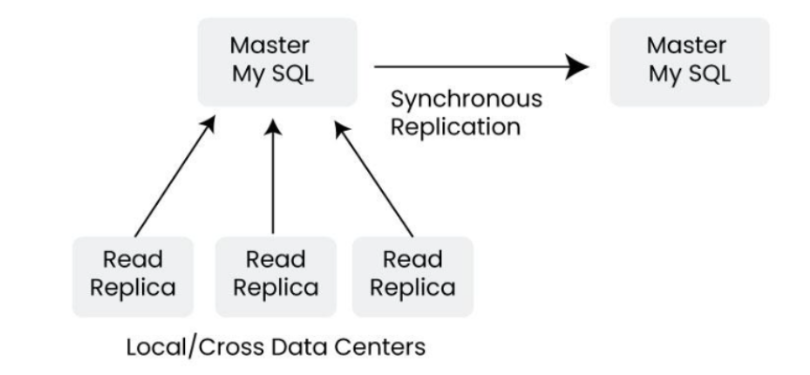
\includegraphics[width=0.8\textwidth]{./img/maestro_maestro_mysql.png}
        \caption{Configuración maestro-maestro de MySQL}
        \label{fig:netflix_mysql}
    \end{figure}

    En este modelo, Netflix opta por una configuración maestro-maestro en MySQL, desplegado en instancias EC2 de Amazon o servidores potentes utilizando el motor de almacenamiento InnoDB para garantizar la integridad de los datos. Esta configuración permite la replicación síncrona entre nodos maestros para que los datos sean consistentes y estén disponibles incluso cuando falle el sistema, mejorando la disponibilidad y la escalabilidad para manejar grandes volúmenes sin reducir el rendimiento óptimo esperado.

    Además, para gestionar estos datos a gran escala, tanto de escritura como de lectura, Netflix utiliza otra base de datos llamada Cassandra, una base de datos NoSQL útil para mejorar la escalabilidad y la alta disponibilidad sin comprometer el rendimiento. Cassandra es especialmente útil para almacenar el historial de visualizaciones de los usuarios, ya que estos crecen exponencialmente a medida que Netflix se expande y obtiene nuevos usuarios.

    El creciente aumento del número de usuarios y, consecuentemente, en el volumen de datos del historial de visualizaciones, Netflix ha tenido que enfrentar el desafío de gestionar correctamente esta creciente demanda. Para ello, implementó una estrategia de almacenamiento que consiste en la comprensión de datos antiguos y el almacenamiento sin comprimir los datos recientes para los trabajos ETL (Extraer, Transformar y Cargar) para reducir la carga del almacenamiento y mantener un rendimiento constante independientemente de si se producen aumentos en las actividades de visualización por parte de los usuarios.

    \begin{figure}[H]
        \centering
        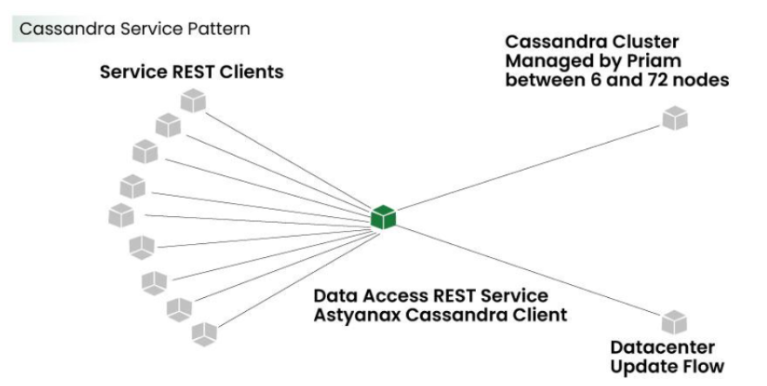
\includegraphics[width=0.8\textwidth]{./img/cassandra_netflix.png}
        \caption{Configuración Cassandra}
        \label{fig:netflix_cassandra}
    \end{figure}

    Por último, cabe mencionar que Cassandra permite a Netflix desplegar una arquitectura distribuida capaz de manejar una gran cantidad de escrituras por segundo, además de permitir copias de seguridad diarias de un tamaño superior a los 30TB y asegurar la disponibilidad de los datos.

    \newpage

    \subsection{Amazon Prime Video}
    Amazon Prime Video ha logrado establecerse como uno de los principales servicios de streaming de video en el mundo, ofreciendo a sus suscriptores una amplia gama de contenido multimedia a través de una plataforma robusta y confiable. En este apartado, exploraremos en detalle la compleja arquitectura tecnológica que sustenta este servicio líder en la industria del entretenimiento en línea.

    \subsubsection{¿Qué debe ofrecer Amazon Prime Video?}

    Entre los requisitos funcionales, se encuentra la necesidad de que los usuarios puedan crear cuentas, iniciar sesión y cerrar sesión de manera eficiente. Además, se requiere una gestión de suscripciones robusta que permita a los usuarios administrar sus preferencias y suscripciones de manera intuitiva.

    Otro aspecto crucial de los requisitos funcionales es la capacidad de reproducción de videos de forma fluida, con opciones como pausar, reproducir, rebobinar y avanzar rápidamente, lo que proporciona a los usuarios un control total sobre su experiencia de visualización. Asimismo, la posibilidad de descargar contenido para verlo sin conexión se considera esencial para adaptarse a las necesidades cambiantes de los usuarios y permitirles disfrutar del contenido en cualquier momento y lugar. \cite{dave2023}

    Por otro lado, los requisitos no funcionales juegan un papel igualmente importante en el diseño del sistema de Amazon Prime Video. Se busca una plataforma sin almacenamiento en búfer o con un mínimo almacenamiento en búfer, con el objetivo de minimizar las interrupciones durante la reproducción de video y garantizar que los videos comiencen rápidamente y se reproduzcan de manera constante. La alta disponibilidad y la coherencia eventual son requisitos clave para asegurar que la plataforma esté siempre disponible y que los servicios proporcionados sean consistentes incluso en situaciones de fallo.

    Además, se establece la necesidad de una aplicación de baja latencia, donde las interacciones del usuario sean respondidas de manera instantánea y la transmisión de video tenga una latencia mínima. Esto se traduce en una experiencia de usuario más atractiva y en tiempo real. Por último, la confiabilidad del sistema es un requisito fundamental, con la garantía de que los videos cargados no se pierdan y se implementen mecanismos sólidos para evitar la pérdida de datos y garantizar la integridad del contenido cargado.

    El diagrama de casos de uso de la plataforma es el siguiente:

    \begin{figure}[H]
        \centering
        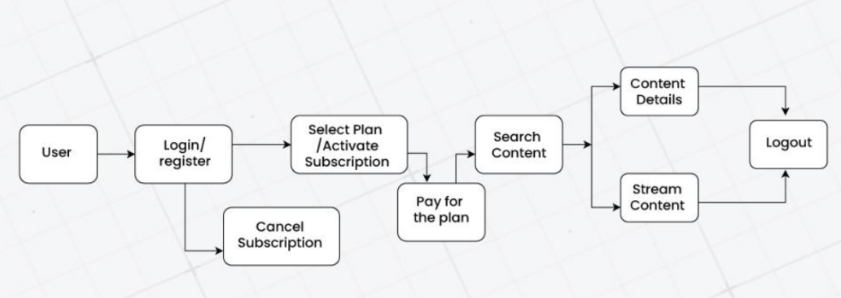
\includegraphics[width=0.8\textwidth]{./img/diagrama_casos_amazon.png}
        \caption{Diagrama de casos de uso de Amazon Prime Video}
        \label{fig:amazon_casos}
    \end{figure}

    \subsubsection{Diseño de bajo nivel del sistema}

    El diseño de bajo nivel del sistema es el siguiente:

    \begin{figure}[H]
        \centering
        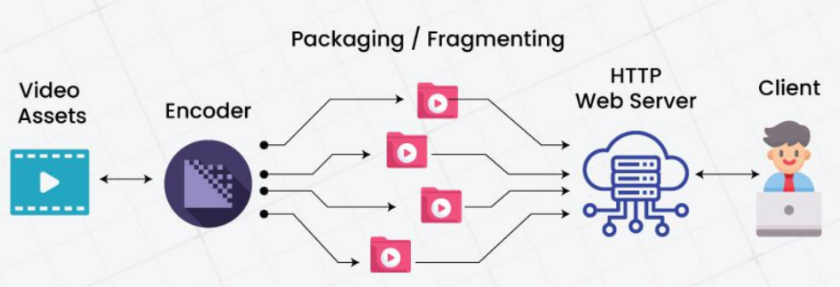
\includegraphics[width=0.8\textwidth]{./img/bajo_nivel_amazon.png}
        \caption{Diseño de bajo nivel de Amazon Prime Video}
        \label{fig:amazon_bajo_nivel}
    \end{figure}

    Los “Video Assets” son el contenido en sí, pudiendo ser una película, documental, serie… Están almacenados en una resolución perfecta en los centros de almacenamiento distribuidos de datos conocidos como Amazon S3 (Simple Storage Service).

    El recurso de video atraviesa un codificador, un componente crucial encargado de comprimir y codificar el video en formatos y tamaños específicos. Este proceso es esencial para la transmisión adaptativa, ya que posibilita que los usuarios reciban video de la máxima calidad conforme a la capacidad de su red. Una vez codificada, la transmisión de video se fragmenta o empaca en segmentos más pequeños. Este procedimiento implica la creación de segmentos de video más compactos que puedan ser transmitidos de manera efectiva a través de Internet. Cada fragmento típicamente representa un breve intervalo del video. \cite{bhasin2024}

    El servidor web HTTP desempeña un papel fundamental en la entrega del contenido de vídeo a los usuarios finales. Almacena y sirve los segmentos de video a los clientes que los solicitan. Cuando un usuario inicia la reproducción, envía solicitudes HTTP al servidor para recuperar los segmentos de video.

    El cliente, que representa el dispositivo o la aplicación del usuario, es responsable de iniciar el proceso de transmisión. Interactúa con el servidor web HTTP para solicitar y recibir segmentos de vídeo. El comprador además administra la lógica de transmisión adaptativa, ajustando dinámicamente la calidad del video según las condiciones de la red del usuario para brindar una experiencia de usuario fluida.

    \subsubsection{Diseño de alto nivel del sistema}

    \begin{figure}[H]
        \centering
        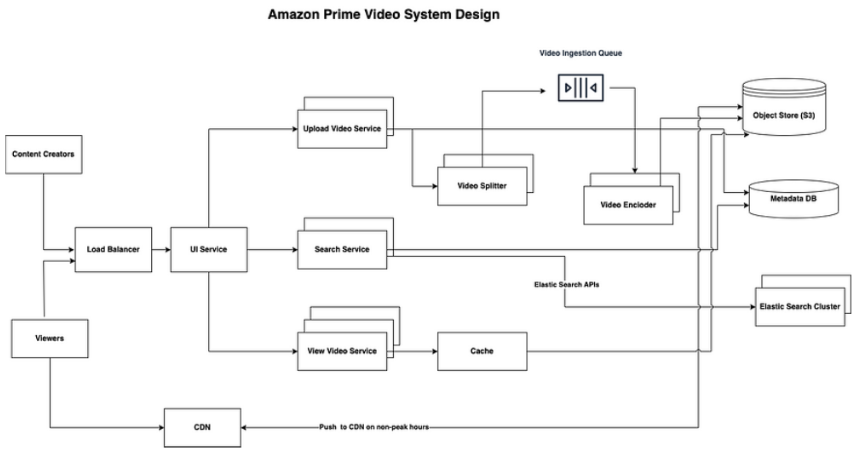
\includegraphics[width=0.8\textwidth]{./img/alto_nivel_amazon.png}
        \caption{Diseño de alto nivel de Amazon Prime Video}
        \label{fig:amazon_alto_nivel}
    \end{figure}

    Los usuarios interactúan con la plataforma Amazon Prime Video a través de varios dispositivos, incluidos teléfonos inteligentes, tabletas, televisores inteligentes o navegadores de Internet. La plataforma está diseñada para brindar una experiencia de usuario uniforme y fluida en diferentes dispositivos.

    El CDN desempeña una función vital en la distribución eficiente de contenido de vídeo a usuarios de todo el mundo. Ayuda a reducir la latencia y acelera la entrega de contenido mediante el almacenamiento en caché de segmentos de video en servidores ubicados estratégicamente. Esto permite una entrega de contenido más rápida a los usuarios, independientemente de su ubicación geográfica.

    El balanceador de carga se encarga de distribuir las solicitudes entrantes de los usuarios entre múltiples servidores para garantizar una distribución uniforme de la carga. Esto mejora la escalabilidad del sistema, la tolerancia a fallas y la utilización de recursos de primer nivel. Esto garantiza que ningún servidor se vea abrumado. \cite{kolny2023}

    Los videos se almacenan, como hemos descrito anteriormente, en los Amazon S3 (Object Store en la Figura 9).

    Cuando los creadores de contenido agregan nuevos videos a la plataforma, el Servicio de carga (Upload Video Service) maneja este servicio. No sólo verifica la integridad del contenido cargado sino que también lo almacena en el sistema de almacenamiento de objetos. Además, actualiza los metadatos asociados con los videos subidos, como el título, la descripción y la duración.

    El View Service es responsable de la experiencia general del usuario. Maneja las solicitudes de los usuarios para la reproducción de videos, garantizando la autorización adecuada. Interactúa con varios servicios para buscar y entregar los segmentos de vídeo necesarios, lo que contribuye a una experiencia de visualización fluida.

    El servicio de división de video divide el video original en segmentos más pequeños y manejables. Luego, estos segmentos se distribuyen para una transmisión eficiente. Este proceso es crucial para optimizar el uso del ancho de banda y garantizar una experiencia de transmisión continua e ininterrumpida. Corresponde a la etapa de Packaging/Fragmenting descrita en el diseño de bajo nivel del sistema de Amazon Prime Video.

    \subsubsection{Arquitectura de microservicios}

    Tal y como hemos visto en ambos diseños, la arquitectura de Amazon Video se subdivide en varios microservicios. Cada microservicio se encarga de una tarea concreta, y luego se comunican entre sí para el correcto funcionamiento de la aplicación a través de APIs.

    \begin{figure}[H]
        \centering
        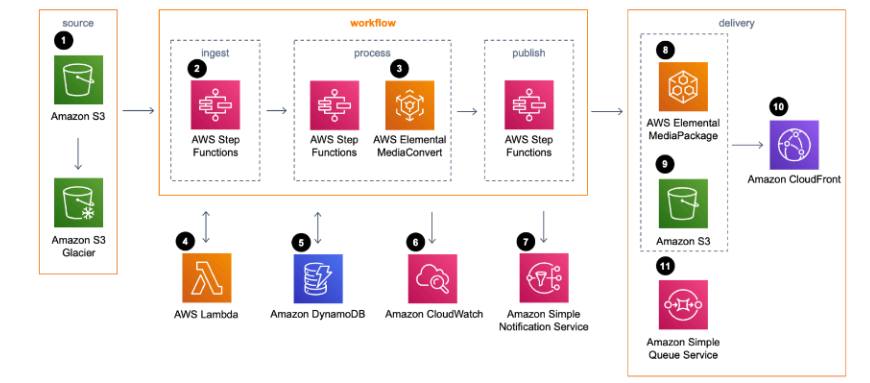
\includegraphics[width=0.8\textwidth]{./img/arquitectura_microservicios_amazon.png}
        \caption{Esquema de la arquitectura de microservicios de Amazon Video}
        \label{fig:amazon_microservices}
    \end{figure}

    Amazon Prime Video aprovecha su servicio de almacenamiento en la nube Amazon S3 para almacenar los archivos de video, apoyándose en otro sistema como es Amazon S3 Glacier, el cual utilizan para almacenamiento de archivos y datos que no suelen ser accedidos con frecuencia, como podrían ser los metadatos de los vídeos, copias de seguridad, o simplemente versiones antiguas.

    Para el procesamiento del vídeo, la transcodificación y adaptación de la resolución y el bitrate utilizan otro microservicio que ofrece AWS, como es AWS Elemental MediaConvert. Este microservicio se apoya además en AWS Step Functions, que no es más que otro microservicio que permite coordinar y orquestar fácilmente las tareas y flujos de trabajo en aplicaciones distribuidas y basadas en la nube. Proporciona una forma visual de diseñar y ejecutar flujos de trabajo que constan de múltiples pasos o etapas.

    Sin embargo, no es el único microservicio que presta apoyo en este flujo de trabajo. Otros, como AWS Lambda, permite ejecutar código de manera automática sin necesidad de aprovisionar o administrar servidores. En Amazon Prime Video es utilizado simplemente para procesar los mensajes de error. Otro apoyo sería Amazon DynamoDB, que se encarga de almacenar datos capturados durante el flujo de trabajo, como pueden ser algunas métricas de rendimiento. Por último, Amazon CloudWatch es un servicio de monitoreo y observabilidad que permite a los usuarios supervisar y gestionar los recursos y aplicaciones en la nube de manera centralizada, por lo que es utilizado para tareas de logging.

    Una vez finalizado el proceso de transcodificación y división del video original, proceso el cual ya hemos remarcado su importancia, se pasa al proceso de entrega del video al usuario. Para ello, se utiliza el servicio AWS Elemental MediaPackage, que facilita la preparación y el empaquetado de contenido de vídeo para la entrega en línea a través de Internet. Está diseñado específicamente para ayudar a los proveedores de contenido a preparar su contenido de video para su distribución en la nube de manera segura, escalable y de alta calidad. Se utiliza para crear secuencias de video formateadas para reproducirse en varios dispositivos desde una única entrada de video y proteger el contenido contra el uso no autorizado mediante el cifrado de contenido y la gestión de derechos digitales.

    Sobre el CDN, Amazon Prime Video utiliza otro microservicio para ello, denominado Amazon CloudFront, que no es más que un servicio de entrega de contenido global proporcionado por Amazon Web Services (AWS), cuyo objetivo principal es distribuir contenido web de manera eficiente con baja latencia y alta velocidad de transferencia a usuarios finales en todo el mundo.

    \subsubsection{Más allá de los microservicios}

    Hasta el momento hemos visto que la división en distintos microservicios es una de las claves para que la aplicación de Amazon Prime Video cumpla con los requisitos tanto funcionales como no funcionales descritos en el apartado 4.2.1.

    Sin embargo, Amazon recientemente decidió cambiar radicalmente la arquitectura de uno de sus microservicios. En concreto se trata del microservicio encargado de inspeccionar la calidad de audio y vídeo, que ha pasado de ser un microservicio serverless, en el que gracias a AWS Lambda se ejecuta código automáticamente en respuesta a una serie de eventos, a una estructura monolito. \cite{ibrahim2023}

    Un monolito es una arquitectura en la que la interfaz de usuario, la lógica del negocio y la interfaz de datos están agrupadas en una sola aplicación. Esta estructura facilita el desarrollo inicial y reduce la repetición de código. Sin embargo, los monolitos pueden volverse difíciles de mantener y escalar a medida que crece la aplicación, y pueden presentar barreras para adoptar nuevas tecnologías.

    \begin{figure}[H]
        \centering
        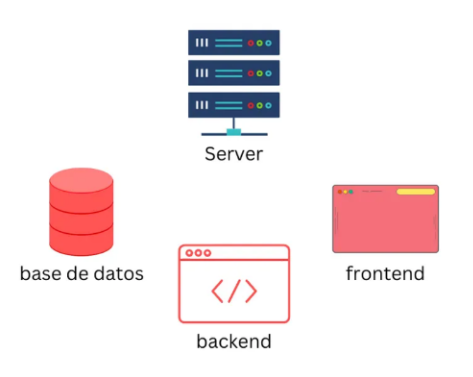
\includegraphics[width=0.8\textwidth]{./img/monolito_amazon.png}
        \caption{Arquitectura de un sistema monolito}
        \label{fig:amazon_monolito}
    \end{figure}

    Inicialmente, la arquitectura de este microservicio encargado de inspeccionar el vídeo y audio era la siguiente:

    \begin{figure}[H]
        \centering
        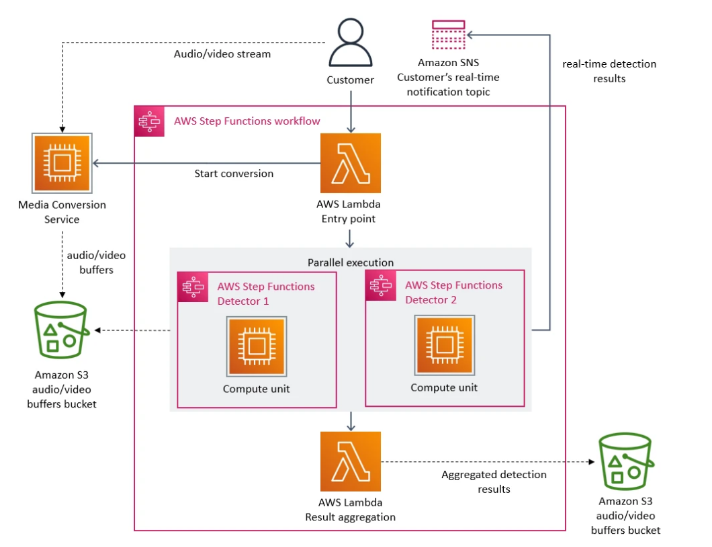
\includegraphics[width=0.8\textwidth]{./img/deteccion_defectos_amazon.png}
        \caption{Arquitectura inicial del sistema de detección de defectos}
        \label{fig:amazon_deteccion_fallos}
    \end{figure}

    Diseñaron su solución inicial como un sistema distribuido que utiliza componentes serverless (microservicios AWS Step Functions y AWS Lambda). Esto supuestamente fue una buena opción para desarrollar el servicio rápidamente. Sin embargo, la utilización ineficiente de algunos componentes les hizo alcanzar un límite de escalado de alrededor un 5\% de la carga esperada. Con todo eso, el coste total de todos los componentes era demasiado alto para aceptar esta solución a gran escala.

    Luego de migrar a monolito la arquitectura quedó de esta forma:
    
    \begin{figure}[H]
        \centering
        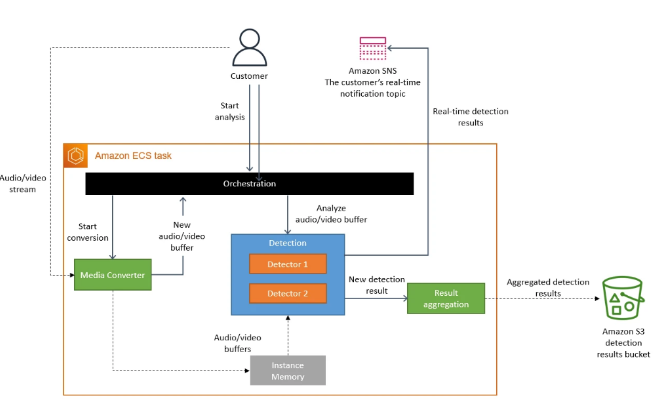
\includegraphics[width=0.8\textwidth]{./img/final_deteccion_fallos_amazon.png}
        \caption{Arquitectura final del servicio de detección de defectos}
        \label{fig:amazon_deteccion_fallos_fin}
    \end{figure}

    Los cambios realizados son los siguientes:

    \begin{itemize}
        \item Combinar todos los componentes en un solo proceso: En lugar de mantener los componentes como microservicios separados, los combinaron en un único proceso. Esto eliminó la necesidad de utilizar un almacenamiento intermedio costoso (Amazon S3) y permitió que las transferencias de datos ocurrieran en la memoria.
        \item Implementar una orquestación simplificada: Al combinar todos los componentes en un solo proceso, la lógica de orquestación se simplificó significativamente. Ya no era necesario utilizar AWS Step Functions para controlar los flujos entre los componentes, lo que redujo los costos y eliminó uno de los principales cuellos de botella.
        \item Utilizar Amazon EC2 y Amazon ECS para la implementación: Al compilar todas las operaciones en un solo proceso, el equipo pudo aprovechar las capacidades de escalabilidad de EC2 y utilizar ECS para administrar estos contenedores. Esto les permitió manejar miles de transmisiones concurrentes y mantener la capacidad de escalar el servicio aún más.
    \end{itemize}

    Debido al cambio radical en la arquitectura del servicio, Amazon ha logrado reducir los costes de infraestructura en un 90\%, además de aumentar sus posibilidades de escalabilidad.

    Esto demuestra que no existe una solución única para todos en cuanto a la arquitectura de software. Aunque los microservicios y serverless pueden funcionar bien a gran escala, la elección entre ellos y un monolito debe tomarse caso por caso.


    \newpage
    
    \subsection{Youtube}

    Para entender cómo funciona la arquitectura de YouTube y el por qué de cada una de sus partes, vamos con una pequeña introducción para luego ir indagando en cada uno de los subsistemas.

    \begin{figure}[H]
        \centering
        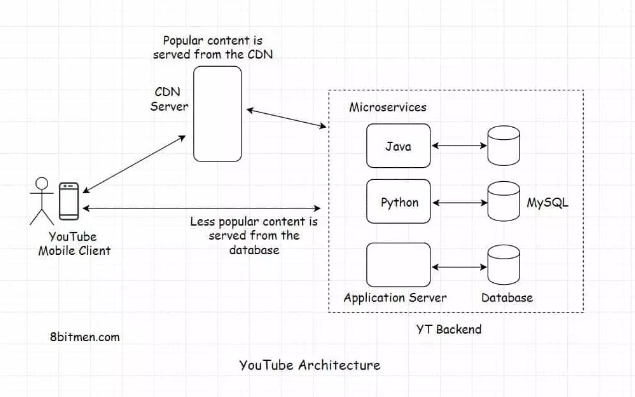
\includegraphics[width=0.8\textwidth]{./img/arquitectura_youtube.png}
        \caption{Arquitectura Youtube}
        \label{fig:arquitectura_youtube}
    \end{figure}

    La arquitectura de Youtube se puede interpretar como cualquier aplicación web en 3 grandes partes:

    \begin{itemize}
        \item \textbf{Front-end:} El frontend, conformado por la aplicación, tal y como la conocemos, con sus canales, sus directos, su zona de foros, comentarios, etc…
        \item \textbf{Back-end:} El backend es la parte más importante de nuestra aplicación de estudio, ya que se suben alrededor de 500 horas de video cada minuto, por lo que tiene que estar muy bien estructurada e implementada, para soportar tal carga de información sin desbordamiento. 
        \item \textbf{Controlador:} Es el que se encarga como ya veremos de suministrar los videos a nuestros clientes, siendo el encargado de distribuirlos según la calidad, mediante los criterios que veremos más adelante. 
    \end{itemize}

    Por lo que ahora vamos a ir punto por punto entendiendo todas las partes que conforman la arquitectura de Youtube. \cite{gfg2023}.
 
    \subsubsection{¿Cómo consigue YouTube almacenar tanta cantidad de información por segundo sin desbordarse?}

    Al principio la base de datos utilizada por la plataforma tenía una sola instancia, pero cuando se incrementaron las QPS (Queries Per Second) se tuvo que ampliar su capacidad de almacenamiento escalando la base de datos de forma horizontal gracias al modelo de base de datos relacional de Vitess. \cite{morrison2022}.

    \subsubsection{Servicio Maestro-Esclavo replica}

    Se instalaron varios modelos antes de llegar al sistema de Vitess, para atajar el problema del aumento de QPS, se instauró el modelo Maestro-Esclavo.

    \begin{figure}[H]
        \centering
        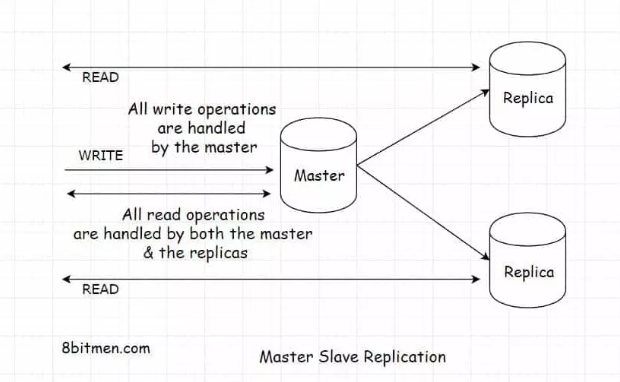
\includegraphics[width=0.8\textwidth]{./img/maestro-maestro_youtube.png}
        \caption{Maestro-Maestro Youtube}
        \label{fig:maestro_maestro_youtube}
    \end{figure}

    La manera que tiene de funcionar el sistema es mediante el reparto de réplicas, cada una de estas réplicas son instancias de bases de datos asociadas a un Maestro, donde este se encargará de gestionar las consultas de escritura. Todas las consultas de escritura pasan por el Maestro, que opera en todas las réplicas, mientras que las consultas de lectura pasan también por las réplicas, para no sobrecargar al maestro y causar un cuello de botella.

    Por la propia estructura del modelo, podría llegar a dar en algunas ocasiones inconsistencia de datos, en situaciones en las que le llegue una operación de escritura al maestro y antes de que éste la ejecute en una determinada réplica donde ya se hayan solicitado una lectura de esa tabla en cuestión, por ejemplo. \cite{shivang2023b}.

    Bueno, esa inconsistencia es aceptable, ya que en un determinado momento luego volverá a ser consistente y al espectador eso no le importa, le es más importante que el video cargue con algunos fallos a que tarde más en cargar. 

    La alternativa Maestro-Réplica no fue más que temporal, debido a que siguieron aumentando las QPS, lo cual no era sostenible con el sistema actual y la cantidad de vídeos subidos por segundos que debía soportar la plataforma. 

    \subsubsection{Sharding}

    La nueva estrategia surgió en trocear la base de datos, lo cual incrementó de forma notable la cantidad de consultas por segundos que se permitían en la base de datos, pero dificultó mucho su mantenimiento y entendimiento de la misma. Además que para confirmar su resiliencia, por cada nueva información que se incluía en esa se tenía que replicar en trozos de servidores hosteados en diferentes máquinas.

    \begin{figure}[H]
        \centering
        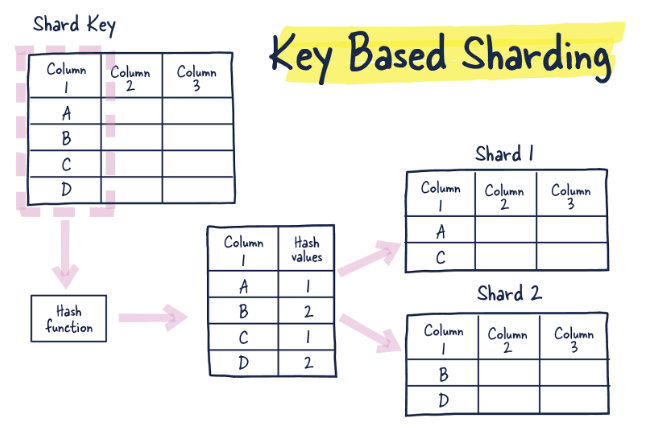
\includegraphics[width=0.8\textwidth]{./img/sharding_youtube.png}
        \caption{Sharding Youtube}
        \label{fig:sharding_youtube}
    \end{figure}

    En la imagen se puede ver bien representado que ahora no solo se cuenta con un maestro que maneje la base de datos si no que tendríamos que duplicar las operaciones en diferentes máquinas con “shared instances”. Por lo que finalmente la solución propuesta por los ingenieros de Youtube fue la de crear Vitess, un sistema de clustering para escalada horizontal de bases de datos MySQL.

    \subsubsection{¿Qué es Vitess?}

    Vitess es una base de datos relacional montada como sistema de clusterización para MySQL, que funciona como sistema que trabaja conjuntamente para permitir que MySQL sea más resiliente, es decir, para que el sistema sea más persistente y pueda recuperarse mejor a fallas e interrupciones inesperadas.

    Se creó en 2010 por un equipo de YouTube para poder incrementar la escalabilidad de la base de datos sobre demanda que era requerida por la plataforma gracias, pero a día de hoy tiene contribuciones de diferentes empresas como Google, GitHub, etc… Ya que es de código abierto. 

    \subsubsection{¿Cómo consigue resiliencia Vitess?}

    En el corazón no se trata más que de otra aplicación MySQL, pero mucho más especializada que otras, su característica principal es que añade más instancias de la aplicación, por lo que si una cae simplemente redirige la carga a otra. 

    Vitess carga varias instancias de MySQL utilizando un proxy denominado VTGate, por lo que detecta de forma automática las instancias offline y redirige al mejor candidato para procesar la query de tabla dada. 

    \subsubsection{Escalabilidad con Vitess}

    Vitess te permite la escalabilidad horizontal con mínimos cambios en la aplicación, puede dividir las tablas a lo largo de diferentes instancias de MySQL, lo que le permite cargarse a lo largo de múltiples servidores.

    Cuando se recibe una consulta por VTGate, el sistema automáticamente determina cuál es la instancia MySQL más adecuada para realizarla y la devuelve como si de una sola instancia se tratara, siguiendo el modelo de caja negra. 

    \begin{figure}[H]
        \centering
        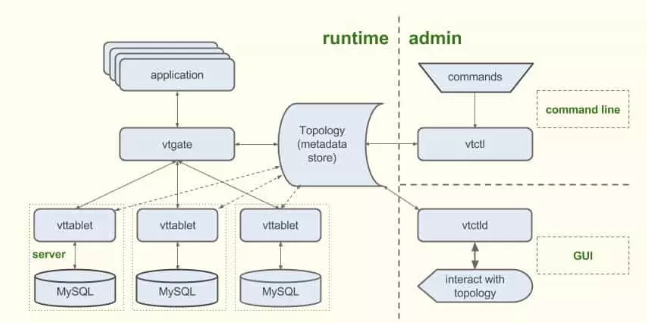
\includegraphics[width=0.8\textwidth]{./img/escalabilidad_vitess.png}
        \caption{Escalabilidad con Vitess Youtube}
        \label{fig:escalabilidad_vitess_youtube}
    \end{figure}

    Este sería un ejemplo de estructura de cómo funciona el sistema de forma gráfica, donde vemos las diferentes instancias de las base de datos MySQL, gestionadas por la vttablet con conexión a la VTGate que es la que controla las conexiones con la aplicación. 

    Cabe destacar que a día de hoy toda la base de datos como cabe esperar está desplegada en los sistemas cloud de Google.

    \subsubsection{CDN}

    El CDN (Content Distribution Network) de Youtube, es uno de los elementos que más ventaja proporciona a YouTube frente a otros distribuidores y plataformas de streaming.

    Youtube usa baja latencia, con un bajo costo asociado, gracias a usar la red global de Google, lo que le permite apalancar su eje de distribución global con los POPs (Points Of Presence), lo que le permite acceder a los clientes a la información desde el server original de la manera más rápida, ya que Google cuenta con servidores alrededor de todo el mundo. 

    \subsubsection{Video Transcoding}

    Uno de los puntos más importantes a tener en cuenta cuando se suben videos a la plataforma, es la transcodificación de videos. Cuando un video se está subiendo a YouTube se renderiza a un formato distinto que el de subida de forma temporal, para que el video se almacene en diferentes formatos, para que el video se pueda reproducir en diferentes dispositivos y anchos de banda.

    Eso permite a YouTube hacer videos en streaming en diferentes resoluciones como: 144p, 240p, 360p, 480p, 720p, 1080p, etc.. Cabe remarcar también que YouTube cuenta con algoritmos que comprimen videos largos en tamaños más pequeños, esta herramienta es denominada Codecs. 

    \subsubsection{YouTube's Video Delivery Architecture}

    Una vez hemos entendido de forma granular cada una de las partes que componen la arquitectura de YouTube, desde el Back hasta los Middleware, podemos hacer una pequeña flujo de operaciones desde que se almacena hasta que se reproduce solicitado por un cliente:

    \begin{enumerate}
        \item Se sube el video, haciendo la debida transcripción de video subiendo las diferentes resoluciones.
        \item Se realiza la comprensión debida mediante el Codecs.
        \item Es almacenado en la base de datos MySQL en Vitess.
        \item Cuando un usuario solicita un vídeo, se comprueba su dispositivo, resolución de pantalla, capacidad de procesamiento y ancho de banda de internet contratado.
        \item Los videos que tienen más demanda son distribuidos mediante el CDN mientras que los que no son directamente mediante conexiones con el Backend. 
    \end{enumerate}

    \begin{figure}[H]
        \centering
        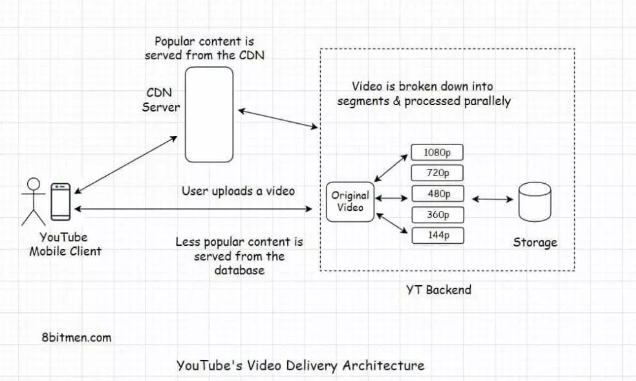
\includegraphics[width=0.8\textwidth]{./img/video_delivery_youtube.png}
        \caption{Video Delivery Youtube}
        \label{fig:video_delivery_youtube}
    \end{figure}


    \newpage

\section{Comparación de las infraestructuras de distintas plataformas}

\subsection{Similitudes en las infraestructuras de Netflix, Amazon Prime Video y YouTube}

Las tres plataformas basan su arquitectura en los microservicios, lo que les permite descomponer sus aplicaciones en servicios más pequeños e independientes que se comunican entre sí a través de APIs. Netflix y Amazon Prime Video se apoyan en AWS, mientras que YouTube lo hace en Google Cloud Services, pero la función que tienen los microservicios dentro de las tres plataformas son muy similares.

Llama la atención que Netflix, principal competidora de Amazon Prime Video, utiliza la colección de microservicios que proporciona AWS, controlada por Amazon. Esto posiciona a Amazon Prime Video en una situación muy favorable en el mercado de las plataformas de streaming, pues en cualquier otro mercado, que la empresa competidora ostente una gran cuota de mercado no es lo deseado. Sin embargo, en esta situación, Amazon es la gran dominadora del mercado. Controla tanto su propia plataforma, Amazon Prime Video, como parte de su principal competidora, Netflix, conociendo detalles de hasta su propia arquitectura e infraestructura.

Para servir el contenido multimedia a los usuarios finales, las tres plataformas hacen uso de un CDN (Content Delivery Network), ya sea propio y desarrollado por ellos mismos o tercerizada con otro microservicio. Debido a la magnitud de las plataformas, su CDN destaca por tener una gran robustez, lo cuál es crucial para minimizar la latencia, mejorar la velocidad de carga de los vídeos y asegurar una experiencia de usuario de alta calidad independientemente de la región geográfica desde la que se realice la petición. \cite{song2021}.

Otro aspecto en el que se asemejan mucho es en el proceso de transcodificación de vídeo. Todas y cada una de las empresas estudiadas consideran este proceso uno de los más importantes de su flujo de trabajo. Además, el input y el output en este proceso es idéntico: se recibe el archivo multimedia y atraviesa un codificador, encargado de comprimir y codificar el vídeo en formatos y tamaños específicos. Este proceso es esencial para la transmisión adaptativa, ya que posibilita que los usuarios reciban video de la máxima calidad conforme a la capacidad de su red. Tras esto, el archivo de vídeo es segmentado en fragmentos más pequeños para que puedan ser envíados a través de la red con menor dificultad.

Por último, debido también a la magnitud de archivos multimedia con los que trabajan cada una de las plataformas, así como el gran número de usuarios, Netflix, Amazon Prime Video y YouTube han diseñado sus infraestructuras para manejar cargas de tráfico muy altas y picos de demanda imprevistos. Utilizan tecnologías de escalabilidad horizontal, como el balanceo de carga y el escalado automático de recursos, para adaptarse dinámicamente a las necesidades de tráfico. \cite{suman2022}.

\newpage


\subsection{Diferencias en las infraestructuras de Netflix, Amazon Prime Video y YouTube}

En cuanto a las diferencias, podemos empezar comentando que Netflix ha desarrollado su propio CDN, que se llama Open Connect, que está diseñado para optimizar la entrega de su contenido, para tener un control directo sobre su distribución y como ofrecen sus servicios.

Sin embargo, Amazon Prime Video se apoya en la propia infraestructura de su compañía AWS, utilizando servicios como Amazon CloudFront para manejar dicha distribución de contenido. Y Youtube, por su parte, utiliza la infraestructura global de Google para utilizar su CDN y servir su contenido de manera eficiente a todos los usuarios del mundo.

En términos de arquitectura, podemos ver que Netflix y Amazon utilizan AWS para el alojamiento de su backend, bases de datos y para gestionar grandes volúmenes de datos. Youtube a diferencia de estas plataformas,  utiliza principalmente la infraestructura de Google Cloud, para computación hasta redes y CDN. 

También debemos comentar que aunque las tres plataformas utilizan una arquitectura de microservicios, Amazon opta por una arquitectura mixta, basado en monolito, para buscar un equilibrio entre agilidad y simplicidad y escalabilidad de su sistema. 

Para la gestión de la calidad del servicio, cada plataforma ha implementado diferentes estrategias, por ejemplo, Netflix utiliza técnicas de resiliencia como los circuit breakers de Hystrix para mantener la estabilidad del servicio, Amazon por su parte, adapta su arquitectura híbrida para mejorar la eficiencia operativa y Youtube, se centra en el uso de algoritmos de compresión avanzados y un sistema de entrega que se ajusta a la demanda de contenido.

Por último, comentar como cada plataforma afronta un enfoque diferente hacia la innovación tecnológica, Netflix utiliza algoritmos de recomendación para mantenerse líder en la personalización de contenido. Amazon Prime integra servicios adicionales, como el e-commerce y Alexa para enriquecer la experiencia del usuario y Youtube opta por ser el pionero en la integración y soporte de formatos de vídeo emergente, como ha ocurrido en estos últimos años con la realidad virtual, ampliando las posibilidades de consumo dentro de su plataforma.

\newpage 
\section{Conclusiones}

Si hacemos una pequeña reflexión, tras haber realizado un pequeño estudio de las plataformas de streaming más grandes, como son Amazon, Netflix y Youtube, a pesar de tener sus diferencias, tienen unas infraestructuras tecnológicas bastante similares para ofrecer sus servicios. 

Ya que aunque utilizan diferentes proveedores de servicios en la nube como puede ser AWS o Google Cloud, la arquitectura que tienen, en general, son bastantes parecidas, dejando como evidencia que aunque haya ciertas características que puedan variar, tienen los mismo fundamentos para la escalabilidad, sostenibilidad y la robustez a nivel del servidor.

Además, algo común en este sector de las plataformas de streaming, es la necesidad de realizar innovaciones tecnológicas para conseguir posicionarse como líder, y como consecuencia en la evolución continua de dichas plataformas. Por ejemplo, Youtube ha tenido que cambiar la base de datos varias veces para intentar adaptarse a los incrementos en la cantidad de contenido, usuarios… etc. \cite{benzina2019}

Finalmente, tras haber realizado un análisis de sus infraestructuras, podemos llegar a la conclusión de que no existe una única manera de alcanzar la escalabilidad, la sostenibilidad y la robustez. Aunque sí es cierto que las arquitecturas pueden ser similares en un diseño de alto nivel, cada empresa utiliza sus estrategias y herramientas tecnológicas para poder cumplir con sus necesidades y maximizar su eficiencia.


\newpage
\section{Bibliografía}

\begin{thebibliography}{99}

\bibitem{adm2023}
Administrador. (2023, 4 noviembre). \textit{Arquitectura tecnológica de Netflix: Conoce el motor de tus maratones de series - Administración de Sistemas}. Administración de Sistemas. Recuperado de \url{https://administraciondesistemas.com/arquitectura-tecnologica-netflix/}

\bibitem{boettger2018}
Böttger, T., Cuadrado, F., Tyson, G., Castro, I., \& Uhlig, S. (2018). Open connect everywhere: A glimpse at the internet ecosystem through the lens of the Netflix CDN. \textit{ACM SIGCOMM Computer Communication Review}, 48(1), 28-34.

\bibitem{gfg2024b}
GfG. (2024b, abril 1). \textit{System design Netflix a complete architecture}. GeeksforGeeks. Recuperado de \url{https://www.geeksforgeeks.org/system-design-netflix-a-complete-architecture/}

\bibitem{hoff2018}
Hoff, T. (2018, 10 febrero). \textit{La compleja infraestructura detrás de Netflix: ¿qué pasa cuando le das al «play»?}. Xataka. Recuperado de \url{https://www.xataka.com/streaming/la-compleja-infraestructura-detras-de-netflix-que-pasa-cuando-le-das-al-play}

\bibitem{dave2023}
Davé, H. (2023, 11 mayo). \textit{Amazon Prime Video Application Architecture: From Micro-services to Monolithic}. Recuperado de \url{https://www.linkedin.com/pulse/amazon-prime-video-application-architecture-from-monolithic-davé/}

\bibitem{bhasin2024}
Bhasin, A. (2024, 24 enero). \textit{Exploring Amazon Prime Video’s Architecture: Migrating from Microservices to Monolith for Audio/Video Monitoring Service}. Medium. Recuperado de \url{https://medium.com/@anshita.bhasin/exploring-amazon-prime-videos-architecture-migrating-from-microservices-to-monolith-for-aacbf9fabc73}

\bibitem{kolny2023}
Kolny, M. (2023, 22 marzo). \textit{Scaling up the Prime Video audio/video monitoring service and reducing costs by 90\% - Prime Video Tech}. Prime Video Tech. Recuperado de \url{https://www.primevideotech.com/video-streaming/scaling-up-the-prime-video-audio-video-monitoring-service-and-reducing-costs-by-90}

\bibitem{ibrahim2023}
Ibrahim, K. (2023, 2 junio). \textit{The Simple Story of Amazon Prime Video’s Bold Transition From Microservices to a Monolith Architecture}. Medium. Recuperado de \url{https://kirillibrahim.medium.com/the-simple-story-of-amazon-prime-video-from-microservices-to-a-monolith-4a1576558e51}

\bibitem{gfg2023}
GfG. (2023, 6 julio). \textit{System Design of Youtube A Complete Architecture}. GeeksforGeeks. Recuperado de \url{https://www.geeksforgeeks.org/system-design-of-youtube-a-complete-architecture/}

\bibitem{morrison2022}
Morrison, B., II. (2022, 21 octubre). \textit{What is Vitess: resiliency, scalability, and performance}. PlanetScale, Inc. Recuperado de \url{https://planetscale.com/blog/what-is-vitess}

\bibitem{shivang2023b}
Shivang. (2023b, octubre 6). \textit{YouTube database – How does it store so many videos without running out of storage space? - ScaleYourApp}. ScaleYourApp. Recuperado de \url{https://scaleyourapp.com/youtube-database-how-does-it-store-so-many-videos-without-running-out-of-storage-space/}

\bibitem{song2021}
Song, M. (2021). A comparative study on over-the-tops, Netflix and Amazon Prime Video: based on the success factors of innovation. \textit{International Journal of Advanced Smart Convergence}, 10(1), 62-74.

\bibitem{suman2022}
Suman, P., Moon, Y. S.,  Choi, M. J. (2022). Netflix, Amazon Prime, and YouTube: comparative study of streaming infrastructure and strategy. \textit{Journal of Information Processing Systems}, 18(6), 729-740.

\bibitem{benzina2019}
Benzina, K. (2019). Cloud Infrastructure-as-a-Service as an Essential Facility: Market Structure, Competition, and the Need for Industry and Regulatory Solutions. \textit{Berkeley Tech. LJ}, 34, 119.

\bibitem{forman2023}
Forman, B. (2023, 15 marzo). \textit{How Prime Video ingests, processes, and distributes live TV to millions of customers around the world, while reducing costs - Prime Video Tech}. Prime Video Tech. Recuperado de \url{https://www.primevideotech.com/video-streaming/how-prime-video-ingests-processes-and-distributes-live-tv-to-millions-of-customers-around-the-world-while-reducing-costs}

\bibitem{puri2023}
Puri, V. (2023, 10 de agosto). \textit{The architecture of the live video broadcast platform on Prime Video}. InfoQ. Recuperado el 17 de abril de 2024, de \url{https://www.infoq.com/news/2023/10/prime-video-availability-costs/#:~:text=The%20architecture%20of%20the%20live,content%20for%20broadcast%20and%20streaming}

\bibitem{shivang2023}
Shivang. (2023, 17 junio). \textit{YouTube Architecture – How does it Serve High-Quality Videos With Low Latency - ScaleYourApp}. ScaleYourApp. Recuperado de \url{https://scaleyourapp.com/youtube-architecture-how-does-it-serve-high-quality-videos-with-low-latency/}




\end{thebibliography}


\end{document}
